\documentclass{beamer}
\usetheme{Berkeley}
\definecolor{UBCblue}{RGB}{25,25,112} % UBC Blue (primary)
\usecolortheme[named=UBCblue]{structure}

\usepackage{ebproof}
\usepackage{forest}
\usepackage{simplebnf}
\usepackage{graphicx}
\usepackage{listings}

\graphicspath{ {./res/} }

\setbeamertemplate{footline}[frame number]

%Information to be included in the title page:
\title{Quelles grammaires permettent la fusion entre analyse syntaxique et analyse sémantique ?}
\author{Enogad Le Biavant--Frederic}
\institute{Alain René Lesage MP2I}
\date{2024}

\begin{document}

\frame{\titlepage}

\section{Présentation générale}
\begin{frame}
		\frametitle{L'idée}
		Karm, 2022
		\begin{center}
				
\includegraphics[scale=0.25]{repo}
		\end{center}
		
\end{frame}

\begin{frame}[fragile]
		\frametitle{L'idée}
		\begin{lstlisting}[language=Lisp]
(defun succ (x) + x 1)
		\end{lstlisting}
		\begin{columns}
				\begin{column}{0.5\textwidth}
						\begin{center}
						\begin{forest}
								for tree = {
										edge = {<-, semithick},
								}
								[succ
										[x]
										[expr
												[+, name=spec +
														[x]
														[1]	
												]
										]
								]
						\end{forest}
						\end{center}
				\end{column}
				\begin{column}{0.5\textwidth}
						\begin{center}
						\begin{forest}
								for tree = {
										edge = {<-, semithick},
								}
								[succ
								[x,edge label={node[midway, left]{$\{x:\tau\}$}}]
										[expr,edge label={node[midway, right]{$\{expr:\beta\}$}}
												[+,edge label={node[midway, right]{$\{\beta = int, \tau = int\}$}}
														[x, edge label={node[midway, left]{$\{x:\tau\}$}}]
														[1]	
												]
										]
								]
						\end{forest}
						\end{center}
				\end{column}
		\end{columns}
												%[DP,draw] {
														%\draw[->,dotted] () to[out=south west,in=south] (spec succ);
												%}
\end{frame}

\section{Définitions}
\subsection{Parsing}
\begin{frame}
		\frametitle{Grammaire}
		\begin{bnf}
				$program$ ::= $expr$;;
				$expr$    ::= | $list$ | $atom$ | $function$;;
				$list$    ::= '(' [\{$expr$\}] ')';;
				$atom$    ::= | $id$ | $literal$;;
				$literal$ ::= | string | int | bool;;
				$function$::= '(' 'defun' $id$ '(' [\{$id$\}] ')' $expr$ ')';;
		\end{bnf} 
\end{frame}

\subsection{Théorie des types}
\begin{frame}
		\frametitle{Définition}
		\begin{center}
				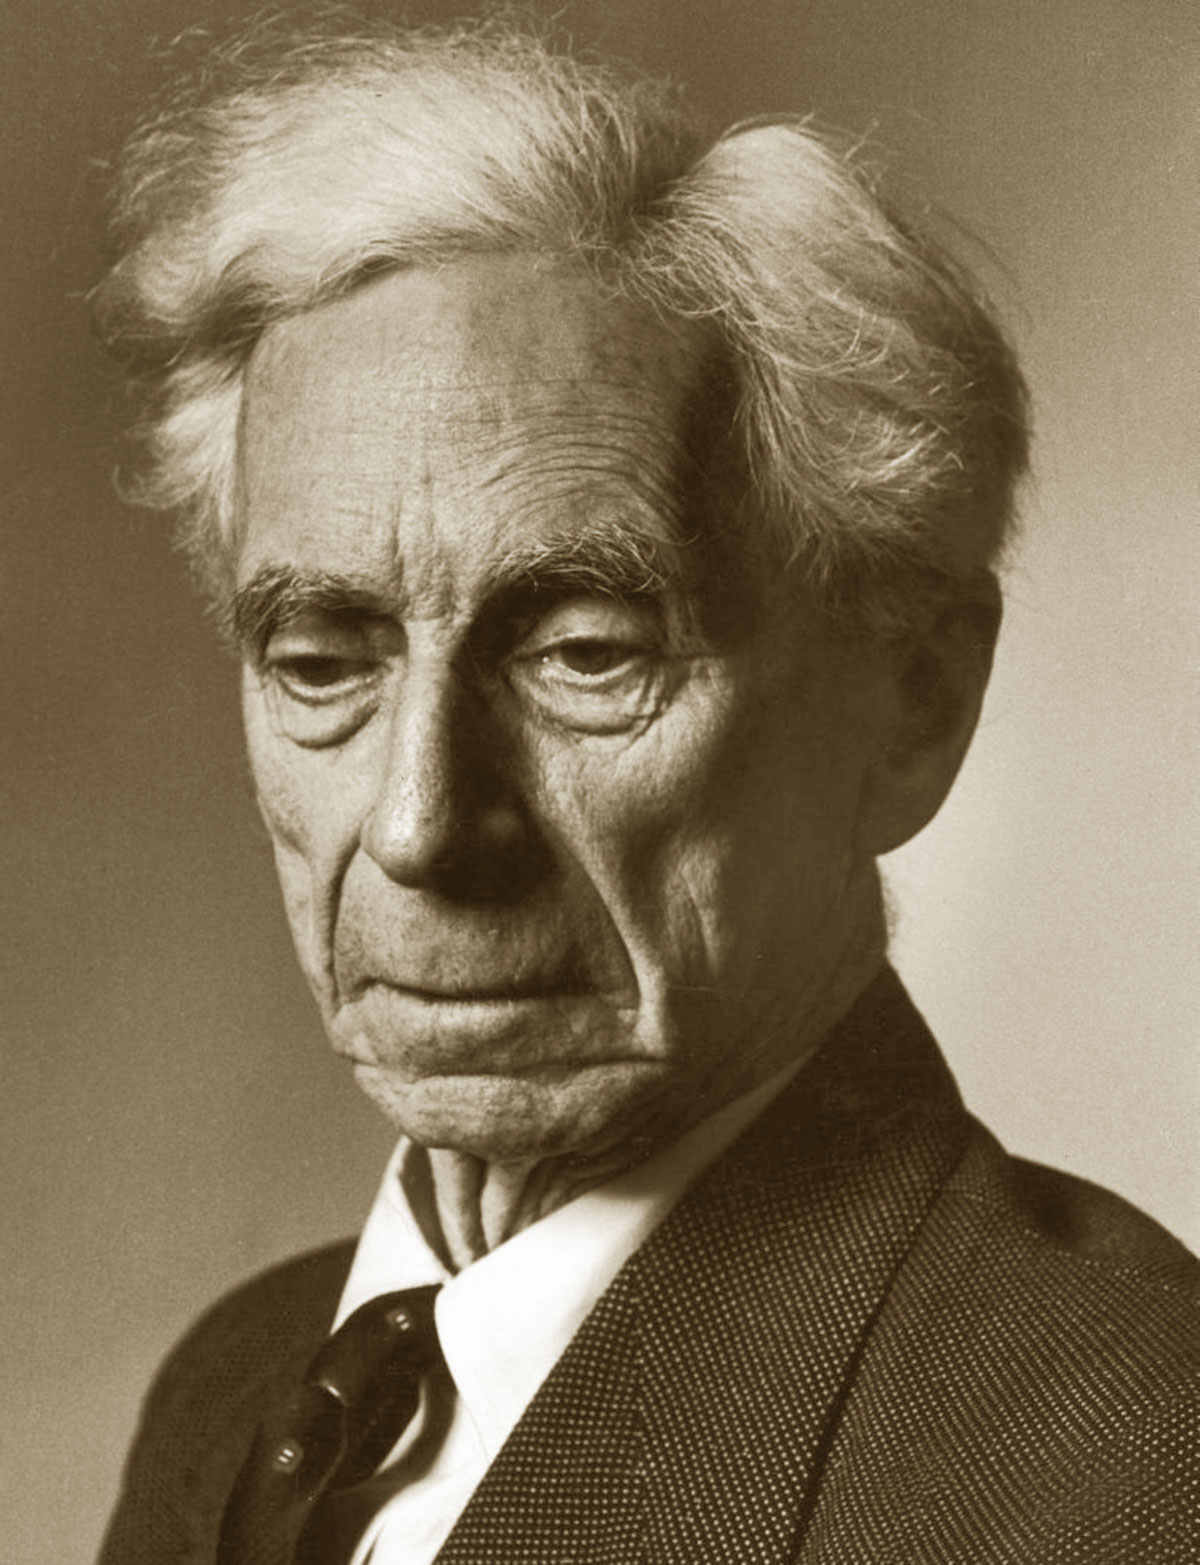
\includegraphics[scale=0.125]{russell}
		\end{center}
\end{frame}

\begin{frame}
		\frametitle{Opérations}
		\begin{center}
				\[
				\begin{prooftree}
						\hypo{A}
						\hypo{B}
						\infer2{C}
				\end{prooftree}
				\]
				\newline
				\[
				A \vdash B
				\]
				\newline
				\[
				\forall \sigma. \sigma\to\sigma
		\]
		\end{center}
\end{frame}

\begin{frame}
\frametitle{Hindley-Milner}
		\[
		\begin{prooftree}
				\hypo{x:\sigma\in\Gamma}
				\infer1[var]{\Gamma \vdash x:\sigma}
		\end{prooftree}
		\]
		\newline
		\[
		\begin{prooftree}
				\hypo{\Gamma, x:\tau \vdash e:\tau'}
				\infer1[abs]{\Gamma \vdash \lambda x.e:\tau \to \tau'}
		\end{prooftree}
		\]
		\newline
		\[
		\begin{prooftree}
				\hypo{\Gamma \vdash f:\tau \to \tau'}
				\hypo{\Gamma \vdash e : \tau}
				\infer2[app]{\Gamma \vdash f\ e : \tau'}
		\end{prooftree}
		\]
\end{frame}

\begin{frame}
		\frametitle{Hindley-Milner}
		\begin{columns}
				\begin{column}{0.5\textwidth}
						\begin{enumerate}
								\item Assignation de variables de types aux expressions
								\item Génération de contraintes
								\item Substitutions
								\item Unification
								\item Instantiation, généralisation
						\end{enumerate}
				\end{column}
				\begin{column}{0.5\textwidth}
						\begin{forest}
								for tree = {
										edge = {<-, semithick},
								}
								[succ
								[x,edge label={node[midway, left]{$\{x:\tau\}$}}]
										[expr,edge label={node[midway, right]{$\{expr:\beta\}$}}
												[+,edge label={node[midway, left]{$\{\beta = int, \tau = int\}$}}
														[x, edge label={node[midway, left]{$\{x:\tau\}$}}]
														[1]	
												]
										]
								]
						\end{forest}
				\end{column}
		\end{columns}
\end{frame}

\section{Ma démonstration}
\begin{frame}[fragile]
		\frametitle{Ma démonstration}
		\begin{lstlisting}[language=Ml]
and parse_atoms (program: Token.t list) (env: Types.env): expr * Token.t list = 
    match program with
    | LParen :: _ -> parse_lists program
    | Id i :: t -> begin
        let s = Types.lookup env i in
        { expr: Atom (Id i); rest: t; env; t: Types.instantiate s; }
    end
    | Literal l :: t -> begin
        match l with
        | Int i -> (Atom (Int i), t)
        | Str s -> (Atom (Str s), t)
        | Bool b -> (Atom (Bool b), t)
    end
    | _ -> failwith "Orphan closing parenthese `RPAREN`"
;;
		\end{lstlisting}
\end{frame}

\section{Et après ?}
\begin{frame}
		\frametitle{Et après ?}
		\begin{itemize}
				\item<1-> Est-ce que il y a un réel impact sur la complexité temporelle ?
				\item<2->Pour quelles grammaires est-ce possible ?
				\item<3->Formalisation de cet outil ?
		\end{itemize}
\end{frame}

\section{Annexe}
\begin{frame}[fragile]
		\frametitle{Annexe}
		\begin{lstlisting}[language=Ml]
let rec substitute s t =
    match t with
    | TVar v -> begin 
        match TypeMap.find_opt v s with
        | Some x -> x
        | None -> TVar v
    end
    | Func (args, ret) -> Func (List.map (substitute s) args, substitute s ret)
    | t -> t
;;

		\end{lstlisting}
\end{frame}

\begin{frame}[fragile]
		\frametitle{Annexe}
		\begin{lstlisting}[language=ml]
let rec unify t1 t2 =
    match (t1, t2) with
    | (Func (args1, ret1), Func (args2, ret2)) when List.length args1 = List.length args2 ->
        let s1 = List.fold_left2 (fun s arg1 arg2 -> 
            compose_subst s (unify (substitute s arg1) (substitute s arg2))
        ) empty_subst_set args1 args2 in
        let s2 = unify (substitute s1 ret1) (substitute s1 ret2) in
        compose_subst s2 s1
    | TVar v, t | t, TVar v -> v |-> t
    | Int, Int | Bool, Bool | Str, Str -> empty_subst_set
    | _ -> raise (TypeError "Cannot unify types")

and (|->) v t =
    (* Binding operation from a type variable to a type (or type variable) *)
    if t = TVar v then empty_subst_set
    else if occurs_check v t then raise (TypeError "Occurs check failed")
    else TypeMap.singleton v t
;;


		\end{lstlisting}
\end{frame}

\end{document}
